\documentclass[10pt]{article}
\usepackage[dvipsnames]{xcolor}
\usepackage{tikz}
\usepackage{url}
\usepackage{multicol}
\usepackage{xspace}
\usepackage{pstricks}
\usepackage{wrapfig}
\usepackage[section]{placeins}
\usepackage{wrapfig}
\usepackage{listings}
\usepackage{textcomp}
\usepackage[default]{droidserif}
\usepackage[T1]{fontenc}

%\usepackage{algorithm2e}
\usetikzlibrary{arrows,automata,shapes}
\tikzstyle{block} = [rectangle, draw, fill=blue!20, 
    text width=2.5em, text centered, rounded corners, minimum height=2em]
\tikzstyle{bw} = [rectangle, draw, fill=blue!20, 
    text width=4em, text centered, rounded corners, minimum height=2em]

\newcommand{\handout}[5]{
  \noindent
  \begin{center}
  \framebox{
    \vbox{
      \hbox to 5.78in { {\bf ECE155: Engineering Design with Embedded Systems } \hfill #2 }
      \vspace{4mm}
      \hbox to 5.78in { {\Large \hfill #5  \hfill} }
      \vspace{2mm}
      \hbox to 5.78in { {\em #3 \hfill #4} }
    }
  }
  \end{center}
  \vspace*{4mm}
}

\newcommand{\lecture}[4]{\handout{#1}{#2}{#3}{#4}{Lab #1}}
\topmargin 0pt
\advance \topmargin by -\headheight
\advance \topmargin by -\headsep
\textheight 8.9in
\oddsidemargin 0pt
\evensidemargin \oddsidemargin
\marginparwidth 0.5in
\textwidth 6.5in

\parindent 0in
\parskip 1.5ex
%\renewcommand{\baselinestretch}{1.25}

\newcommand{\todo}[1]{{\red\textbf{TODO: }#1}\xspace}

\lstset{language=java, 
        basicstyle=\ttfamily,columns=fullflexible,
%	keywordstyle=\color{Blue},          % keyword style
%	commentstyle=\color{OliveGreen}\textit,       % comment style
%	identifierstyle=\color{Black},
%	stringstyle=\color{BrickRed},
	mathescape=true,
	tabsize=3,
	showstringspaces=false}

\begin{document}

\lecture{4 (Navigation)}{Winter 2015}{Kirill Morozov}{version 1.1}

{ \bf Deadline:} You must submit the lab to the SVN repository and be
prepared to demonstrate Lab~4 to a TA by the midpoint of your second assigned
Lab 4 session.  The best way to demo is during a lab session, but any
earlier time where you can convince a TA to watch is OK too.

\begin{figure}[h]
\begin{center}
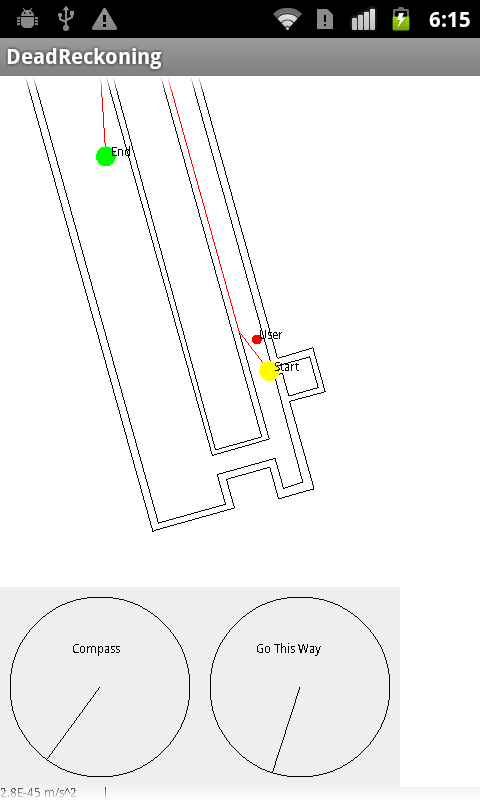
\includegraphics[width=0.25\textwidth]{device-screenshot-lab-4.png}
\end{center}
\caption{\label{fig:lab-4-screen}A complete lab 4 implementation.}
\end{figure}


\section{Objective}
The goal of this lab is to make conclusions about the real world based on sensor data. In particular, you will create an application that reads map information and guides a user through the corresponding physical environment. You will build this application on top of the dead reckoning application from lab 3.

During this lab, you will:
\begin{enumerate}
\item Track the user's position on a model of the physical world.
\item Account for errors in sensor readings based on knowledge of the physical world.
\item Implement a path-finding algorithm which can guide a user to a destination, correcting the user's wrong turns along the way.
\end{enumerate}

\section{Interacting With the Real World}
The {\tt MapView} informs your application when the user changes location or destination, through callbacks. To receive the callbacks, you need to provide a class (possibly your {\tt MainActivity}) implementing the {\tt PositionListener} interface. Call {\tt addListener()} on your {\tt MapView} with a {\tt PositionListener}. The {\tt MapView} will call the {\tt originChanged()} method on your {\tt PositionListener} when the user selects a new starting location, and it will call the {\tt destinationChanged()} method when the user selects a new destination.

The {\tt MapView} also has {\tt setUserPoint()} method, which draws a
red dot at the given location on the map. You will want to call {\tt
  setUserPoint()} immediately whenever {\tt originChanged()} is
called. Similarly, the {\tt MapView} has a method {\tt setUserPath()},
which takes a list of {\tt PointF} objects. It draws this path on the
screen. I recommend using that to show your current heading, that is,
which way your next step will take you on the map.


\paragraph{Utility functions.} Three useful classes are the {\tt NavigationalMap} class,
the {\tt VectorUtils} class, and the {\tt LineSegment} class. {\tt
  VectorUtils} should be familiar to you from high-school linear
algebra; I used {\tt angleBetween} to compute angles between
vectors. {\tt LineSegment} also contains potentially useful methods,
although I didn't use any of them directly. {\tt NavigationalMap}
contains one particularly useful method, {\tt
  calculateIntersections()}, which returns a list of walls between two
{\tt PointF}s.

When comparing numbers which come from the real world and are
potentially jittery, you'll often want to just see if they are ``close
enough'', by seeing if their difference is less than a given
tolerance. It's good design to use a static final field to specify
these tolerances. Locations and angles are numbers that often need to only be
``close enough''.

Keep in mind that our classes operate only in meters. All values should be in meters.

\section{Background}
For this lab, you will need to calculate a route between two points in the presence of obstacles. You do not need to come up with an algorithm from scratch, and may use an existing design, as long as you reference your sources. 

If you choose to use an existing design, please write your own implementation of the algorithm. Do not just copy code from somewhere else.

%% The hardest part of this problem is that you are dealing with a continuous space, so it is difficult to enumerate possible paths. Conceptually, there are two ways of approaching this problem. 

%% \begin{itemize}
%% \item You can accept the continuous nature of the domain and come up with an algorithm that operates on coordinates and directions. In this situation, the number of possible paths is infinite. You will likely be using some heuristics to reduce the solution-space.

%% \item Alternatively, you can reduce the problem to a discrete problem by converting the map into some sort of graph. Once you have reduced the solution-space in this way, you can quite easily use a brute-force solution to enumerate every possible path to the end and then select the best one.
%% \end{itemize}

There are a number of simple-to-implement ways to solve mazes. We'll
start with a simple heuristic and then present two potential full
solutions.

\paragraph{Simple heuristic.} Here's a heuristic that
should work well enough.
\vspace*{-1em}
\begin{itemize}
\item is there a path to the destination free of walls? ({\tt calculateIntersections()} is your
friend here!) If so, take it.
\item no path---then navigate to the first wall between you and the
  destination, and arbitrarily pick an end of the wall to walk
  towards. When the user reaches that end of the wall, your algorithm will calculate
  something different.
\end{itemize}
Such an algorithm should give you almost full marks in this grading scheme, but is not a complete
solution; it gets stuck in corners. You'll get all the marks if you implement a solution that never gets stuck.

\paragraph{Wall-following algorithm.} You can implement a wall-following algorithm.
As long as every wall in the maze touches the edges of the maze, you
can reach the exit from the start by walking forward and keeping your
hand on the left (or right) wall. 

\paragraph{Converting maps into graphs.} 
Physical environments (like rooms) tend to be reasonably simple,
consisting of mostly-straight lines meeting at right angles. You can use
this idea to break up the map into a grid. Each square of the grid
becomes a node in the graph. Nodes are connected to adjacent
nodes as long as there is no intervening wall. 
%Be careful when
%selecting the size of your grid squares. If you make them too small,
%your algorithm will take a long time to run. If you make them too
%large, then a square that straddles two walls may make a passage
%invisible to your algorithm.

You will find that a grid creates many graph nodes which are connected
to all of their neighbours. With a bit of cleverness, you could remove
these nodes or not generate them in the first place.

\paragraph{Magnetic North.}
Be aware that a compass does not point to the north pole (``True North''), but rather to the magnetic north pole. This is the location on Earth where all magnetic field lines point vertically downwards. The maps we provide for use with the mapper will be arranged such that the vertical axis of the map aligns with magnetic north. We mention this because, if you make your own maps, you will need to account for the discrepancy between magnetic and true north.

The way to convert magnetic north into true north is via ``magnetic declination.'' This is the angle between true north and magnetic north. You can consult \url{http://magnetic-declination.com/} to find the magnetic declination of any point on earth. The magnetic declination at Waterloo, Ontario is -9\textdegree\ 41'.

\paragraph{Adjusting for the real world.}
Due to user error and sensor error, any dead reckoning device will slowly drift off course. To correct for this, you can use what you know about the world to correct your calculations. For example, if the algorithm thinks the user just took a step through a wall, which is of course not possible, it should silently drop the step. 

You can detect a wall using {\tt calculateIntersections()} and just a bit of cleverness: calculate the coordinates of the prospective step and see if there are any walls between the current coordinates and the prospective coordinates.

\paragraph{Over-adjusting for the real world.}
You will find that aggressive techniques for taking the real world into account will sometimes cause you to ``get stuck'' on a wall. For example, in the real world, the user may turn a corner, but your application may think that the user was actually two meters behind that. Correcting for this is tricky, so you are not required to do it for this lab.

\section{Demonstration}
Same as with all the previous labs. Don't plagiarize. 
\newpage
\paragraph{Requirements.}
Your app must:
\begin{enumerate}
\item Display the current location of the phone in the {\tt MapView} view, updating after each step.
\item Announce when the destination is reached.
\item Display instructions for the user to reach the destination point selected using the {\tt MapView}. These instructions may take the form of orders (e.g. ``4 steps North and 1 step East''---show which way is north!), or they may take the form of a direction and distance (e.g. ``Walk forward''; ``Turn left by 10 degrees''.) It may be easiest to have a {\tt TextView} which shows the next instruction.
\end{enumerate}
To reduce congestion during testing, we may use a different room for your demo. Your application should support all the rooms for which we provide maps.

We will measure your app on up to three routes, each with between 20 and 30 steps, and give points based on what your algorithm can do. First, we will test your application on a direct route, free of obstacles, from the origin to the destination. You can earn 2 points for this trial by 1) updating the position on the map and 2) pointing the user in the right direction. Next, we will test the behaviour of your application in going around an obstacle. You can earn 1 point on this trial simply by preventing the user position from being inside a wall---the TA will simulate a step through a wall and observe the app's behavious. You can earn 1 additional point by navigating the user along an indirect route which reaches the destination. Finally, on the third trial, the TA will walk in the wrong direction on an indirect route for a while. If your application correctly handles this situation and directs the user to the right destination, you will earn the 1 final mark on the lab, for full marks. In all cases, your application should tell the user when to stop upon reaching the destination.

%We understand that it is hard to be exact when dealing with sensors, especially given that you only have two weeks to write this application. 

It is OK if your application tells the user to cut through corners (but not walls).

For this lab, you will need to convert the number of steps that your pedometer detects into a distance. In our experience this is non-trivial, so you may use one of the following options to make it easier for you, in order of increasing coolness:
\vspace*{-1em}
\begin{itemize}
\item You may hard-code a value. We will provide you with the step lengths for the teaching assistants who will be testing your application.
\item You may add a UI widget where the user may enter a step-length.
\item You may add a calibration mode to your device where you ask the user to walk some number of meters and then count how many steps that takes.
\item You may calculate distance travelled from accelerometer readings.
\end{itemize}
\vspace*{-1em}

%% \paragraph{Bonus}
%% There is a bonus mark associated with this lab.	During testing, you will likely find that sometimes your application's virtual position will ``get caught'' on corners, or will fail to enter hallways. The result of this is that, while the user is moving normally through a hall, the application will think that the phone is still just around the corner. If you can solve this problem, you will earn a bonus mark on this lab.

%% Most solutions will have the position of the user in the {\tt MapView} jump over the wall or corner if the user travels too far in the real world. This should not cause the application to say that the user is inside walls or other unreachable areas.

We have provided you with two different maps of the testing area. One has ``peninsulas'' instead of the tables in the centre of the room---you will find that the wall following algorithm (but not the simple heuristic) is fooled by free standing obstacles. If you can find a way to overcome this problem, you will get a bonus mark. The provided map ``{\tt Lab-room-bonus-destination-and-start.svg}'' shows you two example points that fool basic wall following.

\section{Submission of project files}

Upload the version of your code used in the demo to your subversion repository and commit it. The address is:
\url{https://ecesvn.uwaterloo.ca/courses/ece155/w15/groups/group-NNN-MM}

Email Sanjay Singh if you can't commit to that address.

\section{Tips and hints} 
Compass not working? Make sure that your device isn't in an interfering case.

You'll need to make sure that your app has at least the permission:
\begin{lstlisting}
<uses-permission android:name="android.permission.READ_EXTERNAL_STORAGE" />
\end{lstlisting}
or your app will just crash with a {\tt NullPointerException}. It will also throw a {\tt RuntimeException} if there are no maps in the directory. You may want
to give the app {\tt WRITE\_EXTERNAL\_STORAGE}; that way, it will create 
the appropriate directory for you, and then you can just put the file into that
directory.

If you have points moving when they shouldn't (``Why is my origin
point moving around?''), make sure that you're creating a fresh {\tt
  PointF} object instead of just copying a reference, e.g.  \\ {\tt
  originPoint = new PointF(op.x, op.y); }



You'll find that it will be much easier to develop and
debug your app if you include a button which simulates a step instead
of having to take an actual step. You may want to disable step
detection during development and only enable it for final testing.

\section{Marking scheme} Here's the marking scheme I intend to use. 1 point for each of the following items:
\begin{itemize}
\item updates position on map following steps;
\item finds and presents direct route to destination;
\item does not walk through walls;
\item finds and presents indirect route to destination (going around one obstacle); and
\item compensates for user errors while walking on an indirect route.
\item One additional mark for not getting stuck in corners.
\end{itemize}
We've simplified the default map. If you
use the complex map ({\tt Lab-room.svg} in the repository)
and correctly solve all of navigational challenges without getting
stuck in corners, you will get the final mark.

\end{document}
